\documentclass{article}

\usepackage{amsmath}
\usepackage{booktabs}
\usepackage{calc}
\usepackage{graphicx}
\usepackage{hyperref}
\usepackage{siunitx}
\usepackage{todonotes}
\usepackage{verbatim}

\title{Electronics Lab}

\begin{document}

\listoftodos
\newpage

\maketitle

\todo[inline]{Introduction}
\todo[inline]{Say: students don't have to finish all tasks, nor do they have to
start at the first one}
\todo[inline]{Ensure all figures have suitable captions}

\section{Setup}

On your desk you should find:

\begin{itemize}
\item a breadboard (a white plastic board with a grid of holes)
\item pliers
\item wire strippers
\item wire cutters
\item two LEDs (one red, one green)
\item two resistors
\item a microswitch
\end{itemize}

\todo[inline]{Describe these components in more detail, or add images}
\todo[inline]{Ensure this is up to date}

If some of these items aren't present or if you're having trouble identifying
them, please ask for assistance from one of the mentors.

\subsection{Hookup wire}

We will use single-strand hookup wire to connect up our circuit. Some
electronics kits provide pre-cut wires with connectors attached to each end;
however being able to cut and strip wire off the reel is a good skill to learn.

Using the wire cutters, cut roughly \SI{30}{\centi\metre} of black and red wire
from the reels. Conventially, red wire is used for anything directly connected
to the positive power supply and black wire is used for anything directly
connected to the negative power supply (ground).

Also cut about \SI{60}{\centi\metre} of any other colour. This wire will be used
for any other connections in the circuit. Feel free to use different colours to
represent different sections of the circuit (e.g. blue for input circuitry and
green for output circuitry), or anything else that may help you keep track of
the layout of your circuit better.

Practise cutting a few short lengths of wire and stripping the insulation off
the ends. You should leave between \SI{5}{\milli\metre} and
\SI{10}{\milli\metre} of bare copper at the end; too little and the wire won't
stay securely in the breadboard hole, too much and you risk exposed copper
making contact nearby component leads or other wires and causing a short
circuit. If you are unfamiliar with the process of stripping wires, ask a
mentor to demonstrate the procedure.

\subsection{Breadboard}

In this lab, we will build our circuits on a breadboard, which is a useful
platform for mounting and connecting components that doesn't require soldering.
Some of you may have used a breadboard before; if not, there is an excellent
guide to getting started with breadboards available on SparkFun's website at
\url{https://learn.sparkfun.com/tutorials/how-to-use-a-breadboard}.

The breadboards have two power supply rows at the top, one labelled with
a red line (usually used for the positive power supply) and one with a blue or
black line (for the negative power supply). There are also another two
rows like these at the bottom of the board. Using a piece of (preferably red)
hookup wire, connect the two red rows together. Do the same for the two
black/blue rows with a piece of black wire.

The rest of the holes are the main working area. Each column of five adjacent
holes is electrically connected together.

\subsection{Current, voltage and resistance}

Before we get started on the practical tasks, we need to have some understanding
of how electronic circuits work.

The coulomb (\si{\coulomb}) is the unit of \emph{electric charge}. One coulomb
is equal to the total charge of about \num{6.25e18} electrons. If one coulomb
flows through a wire in one second, then we can say that one ampere of
\emph{current} is flowing. The larger the current in a wire, the more electrons
are moving through it each second.

\emph{Voltage} is what causes a current to flow. When we talk about the voltage
between two points in a circuit, we're referring to how the energy of the
electrons changes as they travel between those points. Batteries are sources
of electrical energy; a \SI{9}{\volt} battery will cause each coulomb of charge
that comes out of one terminal to have \SI{9}{\joule} more energy than when it
went in the other terminal. Most other components are destinations for
electrical energy. For example, a light bulb with a voltage of \SI{12}{\volt}
across it means that each coulomb of charge leaves with \SI{12}{\joule} less
energy than it entered with.

One of the fundamental laws of physics is that energy cannot be created or
destroyed, only transferred. This means that batteries don't create energy;
they simply convert chemical energy to electrical energy. Similarly, motors
convert electrical energy to kinetic energy, and light bulbs convert electrical
energy to light (and thermal energy, if they're not \SI{100}{\percent}
efficient).

Voltage and current are related in many ways; however, perhaps the most
important relationship is Ohm's law. Ohm's law states that the voltage across
a component called a \emph{resistor} is equal to the current flowing through it
multiplied by a constant called the \emph{resistance} of the resistor. In
mathematical notation,

\begin{equation*}
V = I R
\end{equation*}

where $V$ is the voltage, $I$ is the current and $R$ is the resistance. We will
use this equation to help design and analyse our circuits.

\section{Detecting collisions}

A simple way to detect collisions in your robot is to use a circuit involving a
microswitch. 

Let's take a look at the following circuit:

\begin{figure}[h]
\centering
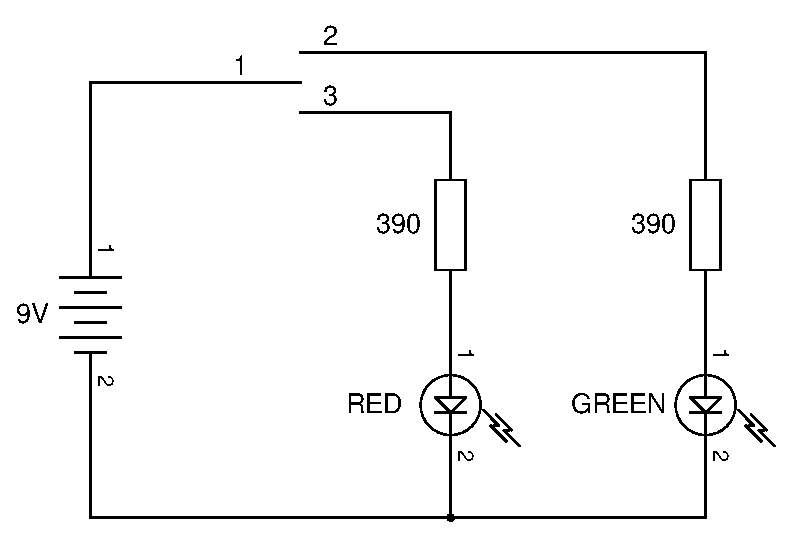
\includegraphics[width=.5\textwidth]{assets/fig/schem/switch}
\label{fig:schem:switch}
\caption{Microswitch circuit. The black rectangle at pin 3 of the switch simply
means that this switch terminal is not connected to anything.}
\end{figure}

When the switch is in the lower position (so that pins 1 and 2 are connected),
the circuit is broken and no current can flow through the resistor. Ohm's law
tells us that the voltage across the resistor is equal to the current times the
resistance; therefore the voltage must also be zero.

If the switch is moved to the upper position (so that pins 1 and 3 are instead
connected), the top end of the resistor is connected to the \SI{3.3}{\volt}
supply. Since the other end is connected to ground (\SI{0}{\volt}), this means
that the voltage across the resistor will be \SI{3.3}{\volt}.

So currently the voltage across the resistor will be either \SI{0}{\volt} or
\SI{3.3}{\volt}, depending on the state of the switch. However, to make this
circuit useful, we want to connect it to our robot's kit. Fortunately, the
JointIO board is designed for interfacing simple electronic circuits to the
robot's central processor. It also provides a handy \SI{3.3}{\volt} power supply
that we can use for our circuit.

Construct this circuit on a breadboard, and connect it to the breadboard as is
shown in Figure~\ref{fig:schem:switch-jointio}. You'll need to know which
microswitch wire is which: \todo{How do wires connect to JointIO? Camcons?}
\todo{Now that we control the colours of the microswitch wires, maybe we should
change to colours that don't violate our convention of ``red is 3.3V, black is
0V''}

\begin{tabular*}{\textwidth}[c]{p{3cm}p{2cm}p{6cm}}
\toprule
Microswitch wire & Pin number on diagram & Description \\
\midrule
Black & 1 & Common \\
Blue & 2 & Connected to common when switch is pressed, disconnected when not pressed \\
Red & 3 & Disconnected when switch is pressed, connected to common when not pressed \\
\bottomrule
\end{tabular*}

\begin{figure}[h]
\centering
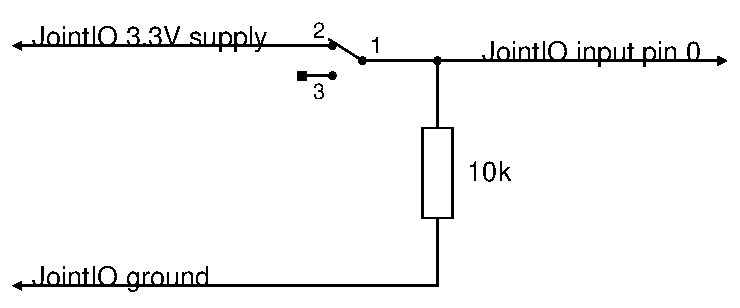
\includegraphics[width=.5\textwidth]{assets/fig/schem/switch-jointio}
\label{fig:schem:switch-jointio}
\caption{Microswitch circuit. The necessary connections to the JointIO board are
shown.}
\end{figure}

\todo[inline]{Think of a corresponding output that can be controlled by this (servo?)}

\todo[inline]{Describe the software side of this.}

\todo[inline]{Say: Why do you think is 10K a good resistor value to use?}
\todo[inline]{Say: How would you modify the setup to turn on the output when
the switch is not pressed (instead of when it \emph{is} pressed)? Can you think
of a solution that only modifies the circuit, and a solution that only modifies
the software?}

\section{Light gates}

Another sensor that may be useful is the \emph{infrared light gate}. In its
simplest form, it consists of two circuits. One powers an infrared LED,
producing a beam of light. A separate circuit then uses a device called a
\emph{phototransistor}, located some distance in front of the LED, to detect if
the beam of light is interrupted before it reaches the phototransistor.

\subsection{The LED circuit}

There are a couple of things to consider when using LEDs in circuits. The first
is their \emph{polarity}, which refers to which way round the two leads are
connected. One of the leads is the \emph{anode} and the other is the
\emph{cathode}. To identify which is which, you can look at either the length of
the leads (the cathode is slightly shorter than the anode) or the lip around the
base of the LED body (which is flat on the cathode's side and curved on the
anode's side). The anode should always be connected to a higher voltage than the
cathode in order for the LED to work.

The other issue is the amount of current flowing through the LED. If it was
connected directly to the power supply, a very large current will flow, which
will almost certainly damage the LED and power supply. Therefore, we will add a
resistor to the circuit to limit the current. The resistor we will use is a
\SI{100}{\ohm} resistor.

Figure~\ref{fig:schem:ir-led} shows the schematic of the LED circuit.

\begin{figure}[h]
\centering
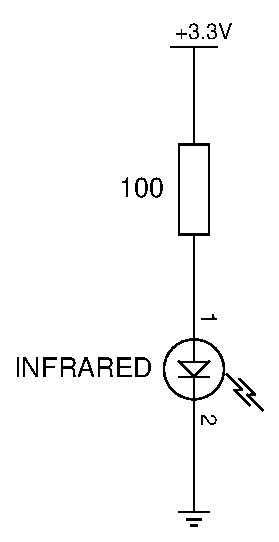
\includegraphics[width=.5\textwidth]{assets/fig/schem/ir-led}
\label{fig:schem:ir-led}
\caption{Light gate LED circuit.}
\end{figure}

The LED has an almost-constant voltage of \SI{1.6}{\volt}, and is rated for a
current of \SI{20}{\milli\ampere}. Work out the voltage across the resistor,
and use Ohm's law to find the current that would flow through the resistor. Is
it less than the LED's current limit?

Construct the circuit on your breadboard, and connect the ground and
\SI{3.3}{\volt} supplies to the corresponding connectors on the JointIO board.
When the circuit is powered up, the LED should emit infrared light. While you
won't be able to see it with the naked eye, a smartphone camera should be able
to detect it.

\subsection{The phototransistor circuit}

A phototransistor is a particular kind of \emph{transistor}. Normal transistors
have three terminals: a collector, a base and an emitter. Transistors function
like switches, in that you can control whether current can flow between the
collector and emitter or not. However, while in a switch this is controlled by
mechanical action, in a transistor it is determined by whether current is
flowing into the base or not\footnote{It's actually a bit more subtle than this;
the larger the base current, the larger the maximum collector-to-emitter
current.} Essentially, it's an electrically-controlled switch.

The key difference between phototransistors and transistors is that
phototransistors don't have an external base pin; instead the switching action
is controlled by whether light is shining on it or not.

Let's examine the circuit we will use for this part of the lab:

\begin{figure}[h]
\centering
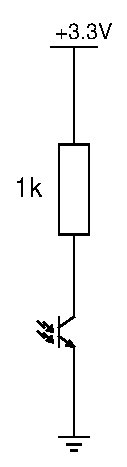
\includegraphics[width=.5\textwidth]{assets/fig/schem/ir-pt}
\end{figure}

When no light is shone on the phototransistor, there is a very high resistance
between the collector and emitter, and so almost no current can flow through
the circuit. As a result of Ohm's law, the voltage across the resistor will be
also be very small. The voltage across the resistor and the voltage across the
phototransistor must always add up to \SI{3.3}{\volt}, so this makes the
voltage across the phototransistor equal to about \SI{3.3}{\volt}.

Now, if light is shone on the phototransistor, then the resistance between the
collector and emitter is much lower, and a large current can flow. Like the LED,
the phototransistor has a roughly constant voltage when it is well illuminated;
for the phototransistor we will be using (a L-53P3C) this voltage is
\SI{0.8}{\volt}. If we use a \SI{1}{\kilo\ohm} resistor, what current will flow
through the circuit? Is this lower than the phototransistor's current rating of
\SI{3}{\milli\ampere}?

In this setup, we will use the JointIO board to measure the voltage across the
phototransistor, since one end of it is connected to ground. We've seen already
that this voltage will be about \SI{3.3}{\volt} if the beam of light is broken,
and about \SI{0.8}{\volt} if it is not. While \SI{0.8}{\volt} is not exactly
equal to zero, it is still less than the threshold voltage\footnote{On the
JointIO board, this threshold voltage is \SI{1.65}{\volt}.} for determining
if an input is ``on'' or ``off''.

\todo[inline]{Describe the software side of this.}

\todo[inline]{Say: Experiment to see how far the LED and phototransistor can be
separated before the system stops working reliably}

\section{Ultrasonic proximity sensors}

\todo[inline]{Depends if we can actually source these}

\section{Controlling a servo}

\end{document}


% Questions:
%   Are bench PSUs available?
%   Are participants working in pairs or on their own?
%   Should hookup wires be provided, or should participants cut and strip their
%    own wire?
%   Do we need to buy pliers, wire strippers etc. or will ECS loan us these?
